\documentclass[handout,nooutcomes]{ximera}
%handout
%wordchoicegiven
%space
%nooutcomes
\title{Math 160 Lab 5}
\author{The Moomaster} 
%\usepackage{todonotes}

\newcommand{\todo}{}

\usepackage{esint} % for \oiint
\graphicspath{
{./}
{functionsOfSeveralVariables/}
{normalVectors/}
{lagrangeMultipliers/}
{vectorFields/}
{greensTheorem/}
{shapeOfThingsToCome/}
}


\usepackage{tkz-euclide}
\tikzset{>=stealth} %% cool arrow head
\tikzset{shorten <>/.style={ shorten >=#1, shorten <=#1 } } %% allows shorter vectors

\usetikzlibrary{backgrounds} %% for boxes around graphs
\usetikzlibrary{shapes,positioning}  %% Clouds and stars
\usetikzlibrary{matrix} %% for matrix
\usepgfplotslibrary{polar} %% for polar plots
\usetkzobj{all}
\usepackage[makeroom]{cancel} %% for strike outs
%\usepackage{mathtools} %% for pretty underbrace % Breaks Ximera
\usepackage{multicol}
\usepackage{pgffor} %% required for integral for loops


%% http://tex.stackexchange.com/questions/66490/drawing-a-tikz-arc-specifying-the-center
%% Draws beach ball
\tikzset{pics/carc/.style args={#1:#2:#3}{code={\draw[pic actions] (#1:#3) arc(#1:#2:#3);}}}



\usepackage{array}
\setlength{\extrarowheight}{+.1cm}   
\newdimen\digitwidth
\settowidth\digitwidth{9}
\def\divrule#1#2{
\noalign{\moveright#1\digitwidth
\vbox{\hrule width#2\digitwidth}}}





\newcommand{\RR}{\mathbb R}
\newcommand{\R}{\mathbb R}
\newcommand{\N}{\mathbb N}
\newcommand{\Z}{\mathbb Z}

%\newcommand{\sage}{\textsf{SageMath}}


%\renewcommand{\d}{\,d\!}
\renewcommand{\d}{\mathop{}\!d}
\newcommand{\dd}[2][]{\frac{\d #1}{\d #2}}
\newcommand{\pp}[2][]{\frac{\partial #1}{\partial #2}}
\renewcommand{\l}{\ell}
\newcommand{\ddx}{\frac{d}{\d x}}

\newcommand{\zeroOverZero}{\ensuremath{\boldsymbol{\tfrac{0}{0}}}}
\newcommand{\inftyOverInfty}{\ensuremath{\boldsymbol{\tfrac{\infty}{\infty}}}}
\newcommand{\zeroOverInfty}{\ensuremath{\boldsymbol{\tfrac{0}{\infty}}}}
\newcommand{\zeroTimesInfty}{\ensuremath{\small\boldsymbol{0\cdot \infty}}}
\newcommand{\inftyMinusInfty}{\ensuremath{\small\boldsymbol{\infty - \infty}}}
\newcommand{\oneToInfty}{\ensuremath{\boldsymbol{1^\infty}}}
\newcommand{\zeroToZero}{\ensuremath{\boldsymbol{0^0}}}
\newcommand{\inftyToZero}{\ensuremath{\boldsymbol{\infty^0}}}



\newcommand{\numOverZero}{\ensuremath{\boldsymbol{\tfrac{\#}{0}}}}
\newcommand{\dfn}{\textbf}
%\newcommand{\unit}{\,\mathrm}
\newcommand{\unit}{\mathop{}\!\mathrm}
\newcommand{\eval}[1]{\bigg[ #1 \bigg]}
\newcommand{\seq}[1]{\left( #1 \right)}
\renewcommand{\epsilon}{\varepsilon}
\renewcommand{\phi}{\varphi}


\renewcommand{\iff}{\Leftrightarrow}

\DeclareMathOperator{\arccot}{arccot}
\DeclareMathOperator{\arcsec}{arcsec}
\DeclareMathOperator{\arccsc}{arccsc}
\DeclareMathOperator{\si}{Si}
\DeclareMathOperator{\proj}{\vec{proj}}
\DeclareMathOperator{\scal}{scal}
\DeclareMathOperator{\sign}{sign}


%% \newcommand{\tightoverset}[2]{% for arrow vec
%%   \mathop{#2}\limits^{\vbox to -.5ex{\kern-0.75ex\hbox{$#1$}\vss}}}
\newcommand{\arrowvec}{\overrightarrow}
%\renewcommand{\vec}[1]{\arrowvec{\mathbf{#1}}}
\renewcommand{\vec}{\mathbf}
\newcommand{\veci}{{\boldsymbol{\hat{\imath}}}}
\newcommand{\vecj}{{\boldsymbol{\hat{\jmath}}}}
\newcommand{\veck}{{\boldsymbol{\hat{k}}}}
\newcommand{\vecl}{\boldsymbol{\l}}
\newcommand{\uvec}[1]{\mathbf{\hat{#1}}}
\newcommand{\utan}{\mathbf{\hat{t}}}
\newcommand{\unormal}{\mathbf{\hat{n}}}
\newcommand{\ubinormal}{\mathbf{\hat{b}}}

\newcommand{\dotp}{\bullet}
\newcommand{\cross}{\boldsymbol\times}
\newcommand{\grad}{\boldsymbol\nabla}
\newcommand{\divergence}{\grad\dotp}
\newcommand{\curl}{\grad\cross}
%\DeclareMathOperator{\divergence}{divergence}
%\DeclareMathOperator{\curl}[1]{\grad\cross #1}
\newcommand{\lto}{\mathop{\longrightarrow\,}\limits}

\renewcommand{\bar}{\overline}

\colorlet{textColor}{black} 
\colorlet{background}{white}
\colorlet{penColor}{blue!50!black} % Color of a curve in a plot
\colorlet{penColor2}{red!50!black}% Color of a curve in a plot
\colorlet{penColor3}{red!50!blue} % Color of a curve in a plot
\colorlet{penColor4}{green!50!black} % Color of a curve in a plot
\colorlet{penColor5}{orange!80!black} % Color of a curve in a plot
\colorlet{penColor6}{yellow!70!black} % Color of a curve in a plot
\colorlet{fill1}{penColor!20} % Color of fill in a plot
\colorlet{fill2}{penColor2!20} % Color of fill in a plot
\colorlet{fillp}{fill1} % Color of positive area
\colorlet{filln}{penColor2!20} % Color of negative area
\colorlet{fill3}{penColor3!20} % Fill
\colorlet{fill4}{penColor4!20} % Fill
\colorlet{fill5}{penColor5!20} % Fill
\colorlet{gridColor}{gray!50} % Color of grid in a plot

\newcommand{\surfaceColor}{violet}
\newcommand{\surfaceColorTwo}{redyellow}
\newcommand{\sliceColor}{greenyellow}




\pgfmathdeclarefunction{gauss}{2}{% gives gaussian
  \pgfmathparse{1/(#2*sqrt(2*pi))*exp(-((x-#1)^2)/(2*#2^2))}%
}


%%%%%%%%%%%%%
%% Vectors
%%%%%%%%%%%%%

%% Simple horiz vectors
\renewcommand{\vector}[1]{\left\langle #1\right\rangle}


%% %% Complex Horiz Vectors with angle brackets
%% \makeatletter
%% \renewcommand{\vector}[2][ , ]{\left\langle%
%%   \def\nextitem{\def\nextitem{#1}}%
%%   \@for \el:=#2\do{\nextitem\el}\right\rangle%
%% }
%% \makeatother

%% %% Vertical Vectors
%% \def\vector#1{\begin{bmatrix}\vecListA#1,,\end{bmatrix}}
%% \def\vecListA#1,{\if,#1,\else #1\cr \expandafter \vecListA \fi}

%%%%%%%%%%%%%
%% End of vectors
%%%%%%%%%%%%%

%\newcommand{\fullwidth}{}
%\newcommand{\normalwidth}{}



%% makes a snazzy t-chart for evaluating functions
%\newenvironment{tchart}{\rowcolors{2}{}{background!90!textColor}\array}{\endarray}

%%This is to help with formatting on future title pages.
\newenvironment{sectionOutcomes}{}{} 



%% Flowchart stuff
%\tikzstyle{startstop} = [rectangle, rounded corners, minimum width=3cm, minimum height=1cm,text centered, draw=black]
%\tikzstyle{question} = [rectangle, minimum width=3cm, minimum height=1cm, text centered, draw=black]
%\tikzstyle{decision} = [trapezium, trapezium left angle=70, trapezium right angle=110, minimum width=3cm, minimum height=1cm, text centered, draw=black]
%\tikzstyle{question} = [rectangle, rounded corners, minimum width=3cm, minimum height=1cm,text centered, draw=black]
%\tikzstyle{process} = [rectangle, minimum width=3cm, minimum height=1cm, text centered, draw=black]
%\tikzstyle{decision} = [trapezium, trapezium left angle=70, trapezium right angle=110, minimum width=3cm, minimum height=1cm, text centered, draw=black]

\outcome{Explain what is meant by the `arc length' of a function.}
\outcome{Describe how to approximate the arc length of a function on a specified interval using a fixed number of line segments.}
\outcome{Give the definition of a smooth function and determine if a particular function is smooth on an interval.}
\outcome{State a formula that gives the arc length of a smooth function on a specified interval.}
\outcome{Determine the arc length of a smooth function using the arc length formula.}
\outcome{Find the arc length of a function that is smooth with respect to y but not x.}
\outcome{Find the arc length of a function that is not smooth at its endpoints but has symmetry.}

\begin{document}

\section{Calculus 1 Lab 5 \\ An Application of Integration - Arc Length}

%% Have to edit the date here each semester.
\begin{abstract}
In this lab, we will explore how we can calculate arc length using a definite integral.  This lab corresponds to section 6.3 in our physical textbook, so feel free to use the textbook as a resource while completing this lab.\\

Unless stated otherwise, input answers in \underline{exact form} on this lab.
\end{abstract}
 
\maketitle

%%Introduction%%

\section {What is arc length and how can it be approximated?}

In the last few weeks of math 160, you will learn about using definite integrals to calculate the areas of 2D regions and volumes of 3D regions.  Integrals can also be used to evaluate the arc length of a function.  Consider the function $f(x) = \sin(x)$ on the interval $[0,2\pi],$ which is graphed below.  \\

\begin{center} 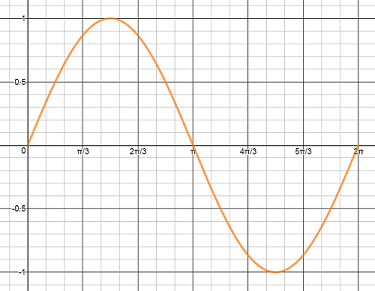
\includegraphics{sinx.png} \end{center}

Imagine laying a string over $f(x)$.  What length of string would you need in order for the string to exactly lay on top of $f(x)$ on the interval $[0, 2\pi]$?  This length is called the `arc length' of the function on the interval $[0, 2\pi]$, and the goal of this lab is to determine how to calculate this length exactly.  \\

At some point in your math education, you probably learned how to calculate the length of an arc on a circle.  The idea of the arc length of a curve is actually the same, except now we would like to calculate the length of \textit{any} curve, not just circular ones.  Aside from circles, you also have the tools to calculate the arc length of a linear function on a particular interval.  For example, consider the function $y = 2x$ graphed below.  Let's find this function's arc length on a few intervals.  

\begin{center} 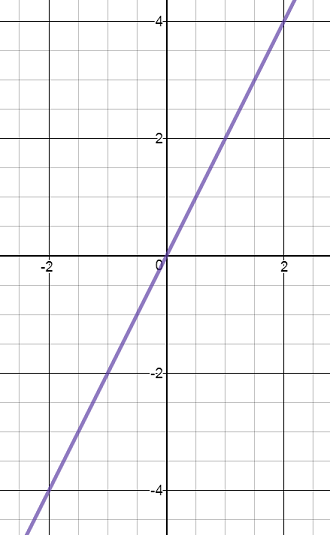
\includegraphics{2x.png} \end{center}

\begin{problem}
Let's first find the arc length of $y$ on the interval $[0,1]$.  Ultimately, this question is equivalent to finding the length of the line segment of $y$ that lies in $[0,1],$ and we know how to find the distance of line segments!  \\ 

The endpoints of this line segment are $(0,\answer{0})$ and $(1,\answer{2}),$ so the $x$-distance between these endpoints is $\Delta x = \answer{1}$ and the $y$-distance between these endpoints is $\Delta y = \answer{2}.$  Notice that a right triangle can be formed with this line segment as a hypotenuse and legs with lengths $\Delta x$ and $\Delta y$, respectively.  Now that we have formed a right triangle, the the Pythagorean Theorem tells us that the length of this line segment and therefore the arc length of $y = 2x$ on the interval $[0,1]$ is $\sqrt{{\answer{1}}^2+{\answer{2}}^2} = \answer{\sqrt{5}}.$
\end{problem}

\begin{problem}
Similarly, we can find the arc length of $y=2x$ on the interval $[-1,2].$  Using the Pythagorean Theorem again, the arc length of $y$ on $[-1,2]$ can be determined to be $\answer{\sqrt{45}}.$
\end{problem}

In a similar fashion, the Pythagorean Theorem could be used to calculate the arc length of \textit{any} linear function on a specific sub-interval and therefore the length of any line segment.  Let's use the fact that we can find the length of any line segment in order to approximate the arc length of the function $f(x) = \sin(x)$ on the interval $[0, 2\pi]$.  Just like we used rectangles to approximate area, let's use line segments to approximate arc length.  For this example, let's use $n=4$ line segments.  Now, we can partition $[0, 2\pi]$ into 4 equal length sub-intervals, $[0, \pi/2]$, $[\pi/2, \pi]$, $[\pi, 3\pi/2]$, and $[3\pi/2, 2\pi]$, and draw a line segment to approximate the arc length on each sub-interval, as shown below.  Finally, to approximate arc length, we must add up the length of these 4 line segments.  Let's do it! \\

\begin{center} 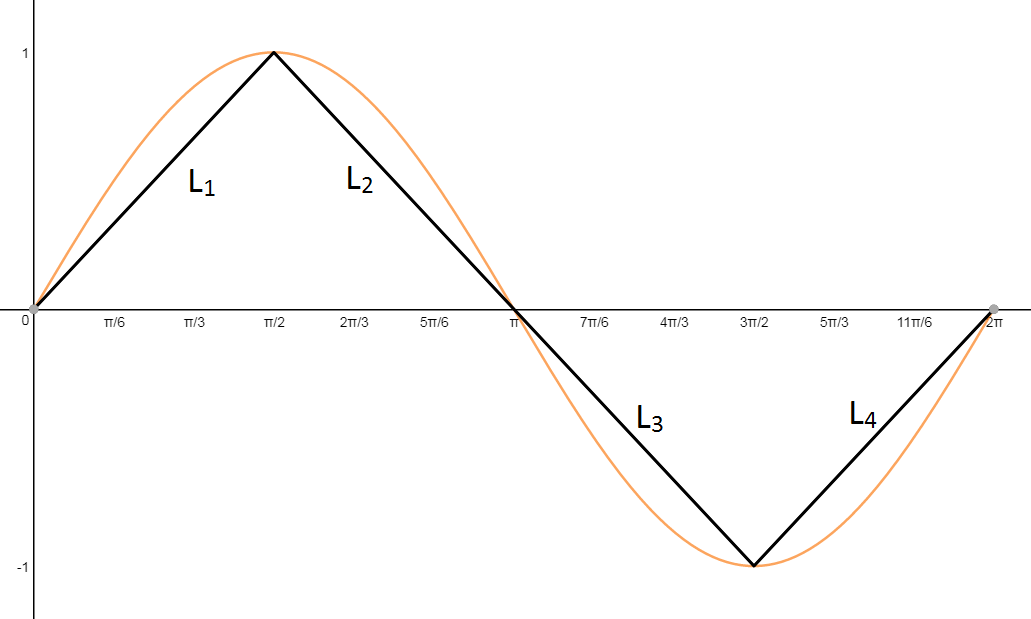
\includegraphics{sinxsegments.png} \end{center}

%%Arc Length Approximation Picture%%

\begin{problem}
Determine the length of each of the four line segments to 2 decimal places.

$L_1 = \answer{1.86}$
$L_2 = \answer{1.86}$
$L_3 = \answer{1.86}$
$L_4 = \answer{1.86}$

So the approximate arc length of $\sin(x)$ on $[0, 2\pi]$ to 2 decimal places is $\displaystyle\sum_{k=1}^4 L_k$ = $\answer[tolerance=0.01]{7.45}.$
\end{problem}

Of course, this is only an approximation of the arc length.  In order to get the \textbf{exact} arc length of $f(x) = \sin(x)$ on $[0, 2\pi]$, we need to take a limit as the number of line segments used ($n$) tends to infinity, just as we did with Riemann sums to calculate exact areas.  To visualize what would happen to the approximation for the arc length of $f(x)=\sin(x)$ on the interval $[0,2\pi]$ as the number of line segments used increases, click on \href{https://www.desmos.com/calculator/lmz7n25cgl}{this link} and drag the slider for $n$.  Notice that as $n$ increases, the sum of the lengths of the line segments is a much better approximation for the desired arc length.  

Because an approximation with $n$ line segments will give an approximate arc length of 

$$\displaystyle\sum_{k=1}^n L_k,$$ 

we can conclude that the exact arc length of $f(x)$ on $[0, 2\pi]$ is given by 

$$\text{Arc Length} = \displaystyle\lim_{n \to \infty} \displaystyle\sum_{k=1}^n L_k.$$  

Unfortunately, we can't evaluate this limit in its current form, so we'll need to write this in another form before we can evaluate this limit and arrive at a formula for the exact arc length.  \\

\section {Deriving a formula for arc length}

Let's move away from $\sin(x)$ for a bit and try to find a formula for the arc length of \textit{any} function $f(x)$ on the interval $[a,b].$  As with the sine example, we can partition the interval $[a,b]$ into $n$ equal length sub-intervals, $[a=x_0, x_1], [x_1, x_2], \dots , [x_{n-1}, x_n = b].$  We will calculate the length of the corresponding line segment that approximates the arc length of $f(x)$ on the kth sub-interval, using the picture below as a guide.  

\begin{center} 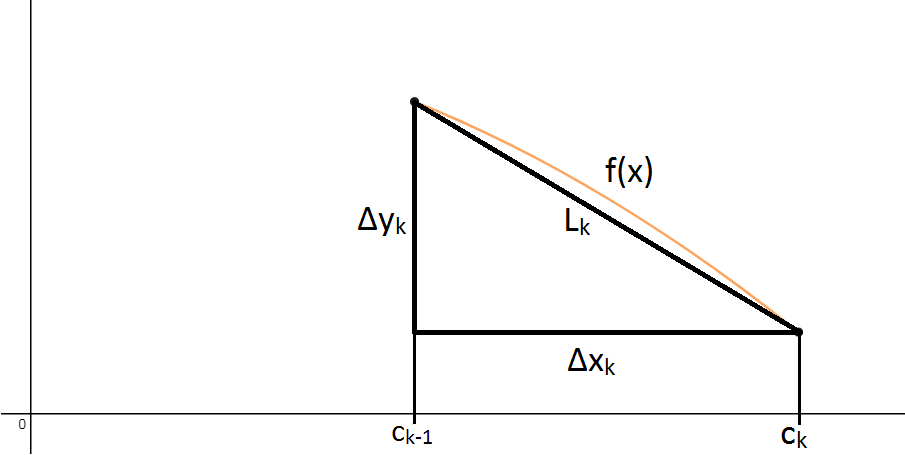
\includegraphics{generalpythagorean.png} \end{center}

The kth line segment being used to approximate the arc length has length $L_k$.  Let's find a way to re-write this length using the Pythagorean Theorem in hopes that this will help us evaluate the previous limit.  Similarly to before, let's denote the $x$-distance between the endpoints of the line segment as ${\Delta x}_k$ and the $y$-distance between these endpoints as ${\Delta y}_k$.  With this notation, $L_k = \sqrt{{{\Delta x}_k}^2+{{\Delta y}_k}^2}$.  Therefore, 

$$\text{Arc Length} \approx \displaystyle\sum_{k=1}^n L_k = \displaystyle\sum_{k=1}^n \sqrt{{{\Delta x}_k}^2+{{\Delta y}_k}^2}.$$

However, we still cannot take the limit of this sum as $n \to \infty$.  Before we can take the limit, we need to re-write this sum once again, this time using the Mean Value Theorem (for derivatives) applied to the kth subinterval.  Recall that this theorem gives a condition under which the average rate of change of a function is equal to the instantaneous rate of change of a function.

\begin{problem}
Specifically, if $f(x)$ is \wordChoice{\choice[correct]{continuous}\choice{differentiable}\choice{integrable}} on $[x_{k-1},x_k]$ and \wordChoice{\choice{continuous}\choice[correct]{differentiable}\choice{integrable}} on $(x_{k-1},x_k),$ then there is some value of $x$ in $(x_{k-1},x_k),$ we'll call it $c_k$, such that $\frac{\Delta y_k}{\Delta x_k} = f'(c_k).$ 
\end{problem}

Solving for $\Delta y_k$, we can now say that on \textbf{every} sub-interval (all $n$ of them), there exists a $c_k$ in $[x_{k-1}, x_k]$ such that

$$\Delta y_k = f'(c_k) \Delta x_k,$$

which allows us to re-write our previous arc length formula as follows:

\begin{align*}
\text{Arc Length} &\approx \displaystyle\sum_{k=1}^n \sqrt{{{\Delta x}_k}^2+{{\Delta y}_k}^2} \\
&= \displaystyle\sum_{k=1}^n \sqrt{{{\Delta x}_k}^2 + (f'(c_k) \Delta x_k)^2} \\
&= \displaystyle\sum_{k=1}^n \sqrt{(1+(f'(c_k))^2)(\Delta x _k)^2} \\
&= \displaystyle\sum_{k=1}^n \sqrt{1+(f'(c_k))^2} \Delta x _k.
\end{align*}

Finally, we have a summation that is similar to the Riemann sums we've calculated in the past in that there is a multiplicative relationship between $\sqrt{1+{f'(c_k)}^2}$ and $\Delta x _k$.  This multiplicative relationship signals that the limit of this sum as $n \to \infty$ is equal to a definite integral!  Therefore, the arc length of $f(x)$ on $[a,b]$ is given by

\begin{align*}
\text{Arc Length} &= \displaystyle\lim_{n \to \infty} \displaystyle\sum_{k=1}^n \sqrt{1+(f'(c_k))^2} \Delta x _k \\ 
&= \displaystyle\int_{a}^{b} \sqrt{1+(f'(x))^2} \ dx .
\end{align*}

What types of functions will this formula apply to?  Well, in order to arrive at this formula for arc length, we had to apply the Mean Value Theorem (for derivatives) to each sub-interval, which required that $f(x)$ is continuous on $[a,b]$ and differentiable on $(a,b).$  Additionally, $\sqrt{1+(f'(x))^2}$ must be integrable or we cannot necessarily evaluate the above integral, so one way to guarantee integrability is to require that $\sqrt{1+{f'(x)}^2}$ is continuous, which occurs precisely when $f'(x)$ is continuous.  Therefore, the above arc length formula applies when $f'(x)$ is continuous on $[a,b]$.  In summary, this formula will apply when 

\begin{itemize}

\item $f$ is continuous on $[a,b],$
\item $f$ is differentiable on $(a,b),$ and
\item $f'$ is continuous on $[a,b]$.

\end{itemize}

However, the condition that $f'(x)$ be continuous on $[a,b]$ implies all of the others, so this is the only condition we need.  This is a very common condition to assume a function satisfies, so functions that satisfy this conditions are given a name.  

\begin{definition}
A function $f(x)$ is \dfn{smooth} on the interval $[a,b]$ when $f'(x)$ is continuous on $[a,b].$
\end{definition}

The reason we call such function \textit{smooth} is because if $f'(x)$ is continuous, then the graph of $f$ will have no discontinuities, corners, or cusps.  If continuous function are considered \textit{nice} functions, then smooth functions are \textit{very nice} functions - after all, not having to worry about corners or cusps in $f$ makes our lives much, much easier.  If you continue learning calculus, you are likely to see smoothness as a hypothesis of many more theorems to come, starting with the following theorem. 

\begin{theorem}[Formula for Arc Length of Smooth Functions]
If $f(x)$ is a smooth function on $[a,b],$ then the arc length of $f(x)$ on the interval $[a,b]$ is equal to 

$$\displaystyle\int_{a}^{b} \sqrt{1+(f'(x))^2} \ dx$$

\end{theorem}

\begin{warning}
Because $\frac{dy}{dx} = f'(x),$ the above formula could also be written as 

$$\displaystyle\int_{a}^{b} \sqrt{1+\left(\frac{dy}{dx}\right)^2} \ dx.$$ 

Be aware that this is the same formula, just written using a different notation for the derivative.  In fact, if you take calculus II, you will return to calculating arc lengths, and you are more likely to see this version of the arc length formula.  
\end{warning}

\section{Practice calculating arc lengths}

%%Practice Problem 1 - Checking sinx Estimate%%

Now that we have derived a formula for the arc length of a curve on a particular interval, let's use this formula to determine the exact arc length of $f(x)=\sin(x)$ on the interval $[0,2\pi]$.  Of course, before using this formula, we must verify that $f(x)=\sin(x)$ is smooth on $[0,2\pi]$.

\begin{problem}

Determine the arc length of $f(x) = \sin(x)$ on the interval $[0, 2\pi].$

$f'(x) = \answer{\cos(x)}$

\begin{problem}

Therefore $f(x)$ is \wordChoice {\choice[correct]{smooth}\choice{not smooth}} on $[0,2\pi]$ because \wordChoice {\choice{f(x) is continuous} \choice[correct]{f'(x) is continuous} \choice{f(x) is not continuous} \choice{f'(x) is not continuous}} on $[0,2\pi]$.  

\begin{problem}

Finally, we can write an integral to evaluate the arc length of the curve on the specified interval and evaluate it using technology.  Our original approximation of this arc length with $n=4$ line segments was 7.45, which turns out to be pretty close to the exact value.  

Arc Length = $\displaystyle\int_{\answer{0}}^{\answer{2\pi}} \sqrt{1+{\(\answer{\cos(x)}\)^2}} \ dx \approx \answer{7.64}$ (Evaluate the arc length to 2 decimal places with technology)


\end{problem}
\end{problem}
\end{problem}

Let's try calculating the arc length of another function.  This time, you will be able to evaluate the resulting integral for arc length by hand using the techniques we've learned in class.

%%Practice Problem 2 - Standard WRT x%%

\begin{problem}

Find the exact arc length of $y = x^{\frac{3}{2}}$ from $x=0$ to $x=4$.  First, we determine if $y$ is smooth on the x-interval $[0,4]$.  

$y' = \answer{\frac{3}{2}\sqrt{x}},$ so $y$ is \wordChoice{\choice[correct]{smooth}\choice{not smooth}} on $[0,4]$ because \wordChoice {\choice{y is continuous} \choice[correct]{y' is continuous} \choice{y is not continuous} \choice{y' is not continuous}} on $[0,4]$.  

\begin{problem}

Arc Length = $\displaystyle\int_{\answer{0}}^{\answer{4}} \answer{\sqrt{1+\frac{9x}{4}}} \ dx = \answer{\frac{8}{27}(10^{\frac{3}{2}}-1)} \ \approx 9.07$ (Evaluate the arc length exactly)

\end{problem}
\end{problem}

The formula for arc length that we derived earlier also applies to functions of $y$ as long as one integrates with respect to y, rather than x.  

\begin{theorem}[Formula for Arc Length of Smooth Functions (of y)]
If $g(y)$ is a smooth function on the y-interval $[c,d],$ then the arc length of $g(y)$ on $[c,d]$ is equal to 

$$\displaystyle\int_{c}^{d} \sqrt{1+(g'(y))^2} \ dy$$

\end{theorem}

Here's an example.  

%%Practice Problem 3 - WRT y%%

\begin{problem}
Find the arc length of $x = \frac{2}{3} (y-1)^{\frac{3}{2}}$ from $y=1$ to $y=4$.  As usual, we must first check that this function of $y$ is smooth on the $y$-interval $[1,4]$.  

$x' = \answer{\sqrt{y-1}},$ so $x$ is \wordChoice{\choice[correct]{smooth}\choice{not smooth}} on the y-interval $[1,4]$.

\begin{problem}
Therefore, because $x$ is smooth, we can determine its arc length on $[1,4]$.

Arc Length = $\displaystyle\int_{\answer{1}}^{\answer{4}} \answer{\sqrt{y}} \ d\answer{y} = \answer{\frac{14}{3}}$ (Evaluate the arc length exactly)

\end{problem}

\end{problem}

Sometimes even if a function $f(x)$ is not smooth, there are still ways to use the arc length formula we derived, as the last few examples will illustrate.

%%Practice Problem 4 - Integrating WRT y When $f$ isn't smooth WRT x%%

\begin{problem}
Find the arc length of $f(x) = \left(\frac{x}{2}\right)^{\frac{2}{3}}$ on $[0,2]$.  

As usual, let's check if $f(x)$ is smooth on $[0,2]$ to determine if the arc length formula applies.

$f'(x) = \answer{(\frac{1}{3})(\frac{2}{x})^{\frac{1}{3}}}.$ 

Therefore, $f(x)$ is \wordChoice {\choice{smooth}\choice[correct]{not smooth}} on $[0,2]$ because \wordChoice {\choice{y is continuous} \choice{y' is continuous} \choice{y is not continuous} \choice[correct]{y' is not continuous}} on $[0,2]$.  

\begin{problem}
In this case, $f'(0)$ does not exist, so $f(x)$ is smooth on $(0,2]$ but not $[0,2]$.  Since $f(x)$ is not a smooth function of $x$ on the interval $[0,2]$, we cannot use the arc length formula in terms of $x$.  However, we can still determine the arc length if $f(x)$ can be written as a smooth function of $y$.  Let's try this and see if we get lucky.  

Written as a function of $y$, $f$ becomes $x = \answer{2y^{\frac{3}{2}}}$ and the $y$-interval that corresponds with the $x$-interval $[0,2]$ is $[0, \answer{1}]$.  

\begin{problem}
From this, we see that $x' = \answer{3\sqrt{y}}$, so $x$ is \wordChoice {\choice[correct]{smooth}\choice{not smooth}} on $[0,1]$.  

\begin{problem}
Now we can use the arc length formula (\textbf{with respect to y}) in order to evaluate the desired arc length of $f(x).$

Arc Length = $\displaystyle\int_{\answer{0}}^{\answer{1}} \answer{\sqrt{1+9y}} \ d\answer{y} = \answer{\frac{2}{27}(10^{\frac{3}{2}}-1)} \ \approx 2.27$ (Evaluate the arc length exactly)

\end{problem}
\end{problem}
\end{problem}
\end{problem}

%%Practice Problem 5- Using symmetry when $f$ isn't smooth WRT x%%

Let's try one last arc length problem involving a non-smooth function.  Let's determine the exact arc length of $f(x) = \sqrt{9-x^2}$ on the interval $[-3,3]$, the graph of which is displayed below.

\begin{center} 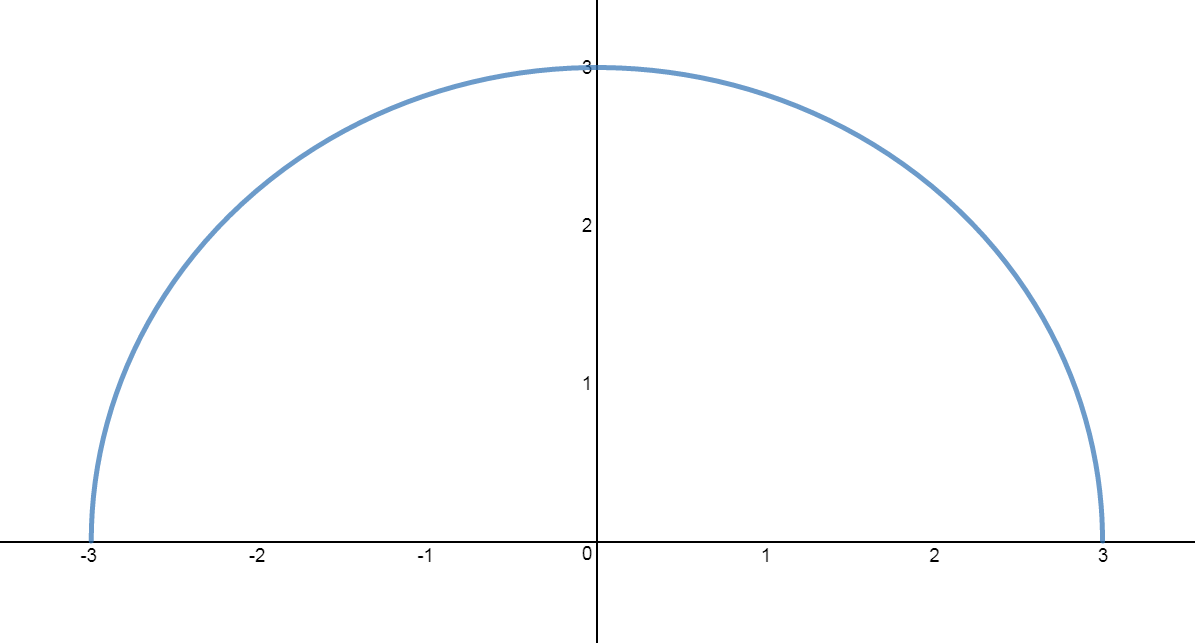
\includegraphics{semicircle.png} \end{center}

\begin{problem}
First off, notice that $f(x)$ is not smooth on $[-3,3]$ because (select all that apply)
\begin{selectAll}
    \choice{f(-3) does not exist.}
    \choice{f(3) does not exist.}
    \choice{f is not continuous at $x=-3$.}
    \choice{f is not continuous at $x=3$.}
    \choice[correct]{f'(-3) does not exist.}
    \choice[correct]{f'(3) does not exist.}
    \choice{f' is not continuous on $(-3,3)$.}
    \choice[correct]{f' is not continuous at the endpoints of $[-3,3]$.}
\end{selectAll}
\end{problem}

Since $f$ isn't smooth on $[-3,3]$, the arc length formula does not apply.  Why not?  Well, $f'(x) = -\frac{x}{\sqrt{9-x^2}}$, so if the arc length formula did apply, we would need to evaluate 

$$\displaystyle\int_{-3}^{3} \sqrt{1+\frac{x^2}{9-x^2}} \ dx.$$ 

The integrand of the above integral has the following graph on the interval $[-3,3].$  \\

\begin{center} 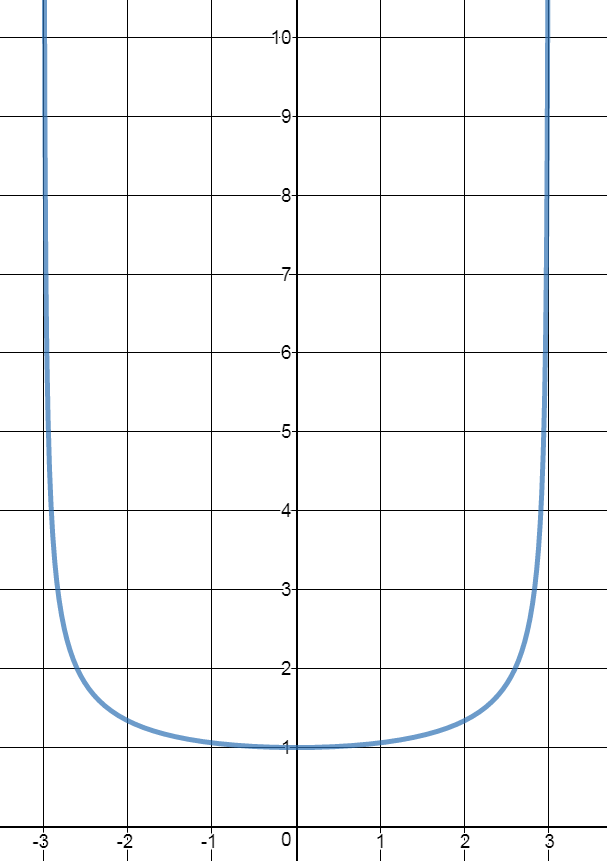
\includegraphics{asymptotes.png} \end{center}

Notice that this integrand has vertical asymptotes at $x=-3$ and $x=3$, so there is no guarantee that the area bounded between $\sqrt{1+\frac{x^2}{9-x^2}}$ and the $x$-axis will converge to a particular number.  In other words, it's possible that this integral cannot be evaluated, despite the fact that the arc length of $f(x)$ can certainly be calculated - $f(x)$ is the graph of a semi-circle after all.  This is one instance of why the arc length formula can only be applied when $f(x)$ is smooth on $[-3,3]$.  Luckily, because $f$ is semi-circular, we do not need calculus to find its arc length.

\begin{problem}
Use the fact that $f(x) = \sqrt{9-x^2}$ is the graph of a semi-circle to evaluate the arc length of $f$ on $[-3,3]$ without using calculus.  

The arc length is exactly $\answer{3\pi}.$
\end{problem}

\end{document}
